\chapter{Conclusion}
\label{ch:conclusion}

\section{Safe Flight Corridor Path Following}

Before we conclude, it is desirable to combine both of the major contributions of this paper, specifically a trajectory following controller for an eVTOL and a path planning algorithm based on RRT to create safe flight corridors. 
A combination of these two contributions is for an eVTOL aircraft to traverse a trajectory generated over an obstacle field by the RRT Safe Flight Corridor algorithm. 
This will test whether the aircraft is capable of following a more complex shape than the simple root trajectories described earlier.

A 2D obstacle field was generated using the RRT algorithm on the North-Down plane. 
The start position was the origin and the end position was $(2000.0, 1000.0)$. 
Nine cubical obstacles of width $100.0$ were placed on a $3 \times 3$ grid. 
The RRT algorithm generated a smoothed SFC path, which is shown in Fig. \ref{fig:SFC_PathFollowing}. 
A video following the aircraft through the trajectory is found at: \href{https://youtu.be/hqRK5J1TDWM}{https://youtu.be/hqRK5J1TDWM}.

\begin{figure}
    \centering
    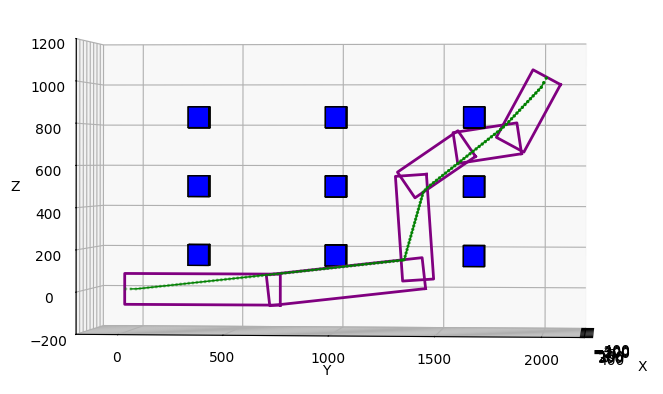
\includegraphics[width=0.95\linewidth]{figs/chap5/PossiblyGoodMap2.png}
    \caption{Safe flight corridor path though $3\times3$ grid, with a B-Spline path generated through it as a flight path reference trajectory. Using the controller from \ref{ch:VTOL}, a VTOL successfully follows this trajectory.}
    \label{fig:SFC_PathFollowing}
\end{figure}

In this case, the aircraft was able to track the generated trajectory and remain withing the safe flight corridors.
The plots of various metrics for the flight are shown in Fig. \ref{fig:RRTControllerMetrics}.

\begin{figure}[htbp]
    \centering
    \begin{subfigure}{0.48\textwidth}
        \centering
        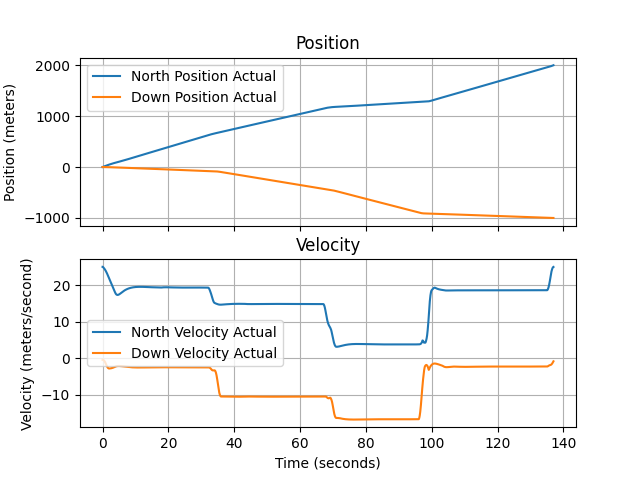
\includegraphics[width=\linewidth]{figs/chap5/ActualPositionVelocity.png}
        \caption{Actual position and velocity of the 2D quadplane over the trajectory. Includes north and down components of position and velocity.}
        \label{fig:ActualPosVelRRT}
    \end{subfigure}
    \hfill
    \begin{subfigure}{0.48\textwidth}
        \centering
        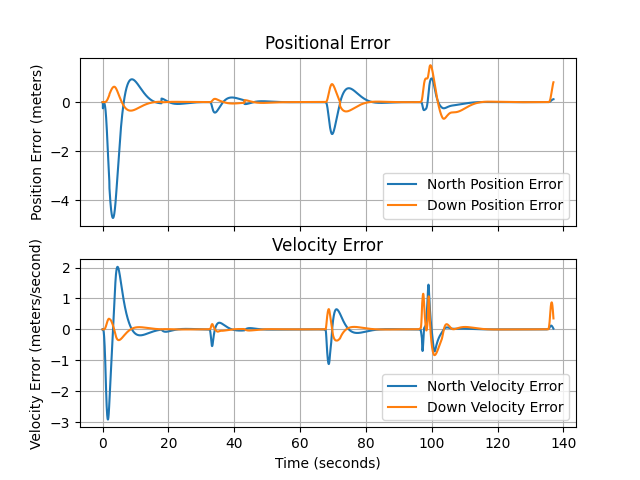
\includegraphics[width=\linewidth]{figs/chap5/PosVelError.png}
        \caption{Position and velocity error of the 2D quadplane, with reference to the 2D trajectory. Includes north and down components of position and velocity.}
        \label{fig:ErrorPosVelRRT}
    \end{subfigure}

    \vspace{0.5cm}  % vertical spacing between rows

    % Row 2
    \begin{subfigure}{0.48\textwidth}
        \centering
        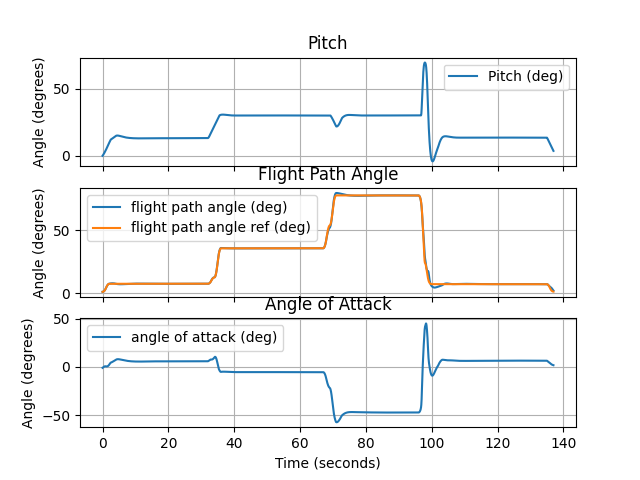
\includegraphics[width=\linewidth]{figs/chap5/Angles.png}
        \caption{Angles of the arcraft through the trajectory. Includes pitch $\theta$, flight path angle $\gamma$, and angle of attach $\alpha$}
        \label{fig:AnglesRRT}
    \end{subfigure}
    \hfill
    \begin{subfigure}{0.48\textwidth}
        \centering
        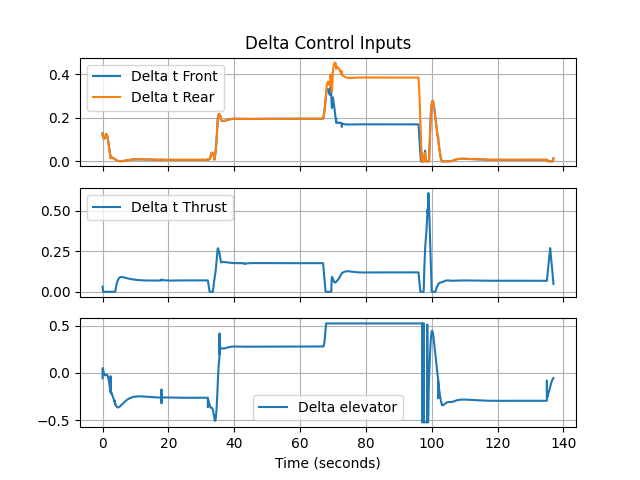
\includegraphics[width=\linewidth]{figs/chap5/Deltas.png}
        \caption{Control inputs $\bs{\delta}$ for the quadplane over the trajectory. Includes forward throttle, vertical throttles, and elevator commands.} 
        \label{fig:deltasRRT}
    \end{subfigure}  
    
    \caption{Metrics for VTOL performance over trajectory generated by 2D RRT SFC algorithm.}
    \label{fig:RRTControllerMetrics}
\end{figure}


\subsection{Controller Failure}

In the previous case, there were no descending sections of the trajectory, and the aircraft was able to follow the trajetory.
Unfortunately, the landing problem, as described in section \ref{sec:landing}, applies to virtually all descending trajectories where a large initial forward velocity is present.
Due to the absence of reverse thrust, the aircraft is unable to stop in its forward velocity.
A map going from an altitude of $1000.0$ meters to $0.0$ meters is shown in Fig. \ref{fig:SFC_PathFollowing_failure}.
A video showing the failed flight may be found at \href{https://youtu.be/eCK1mhtVeUE}{Descent Failure}.
Again, this demonstrates the need for a modification to the control allocation section of the controller to account for this anomaly.

\begin{figure}
    \centering
    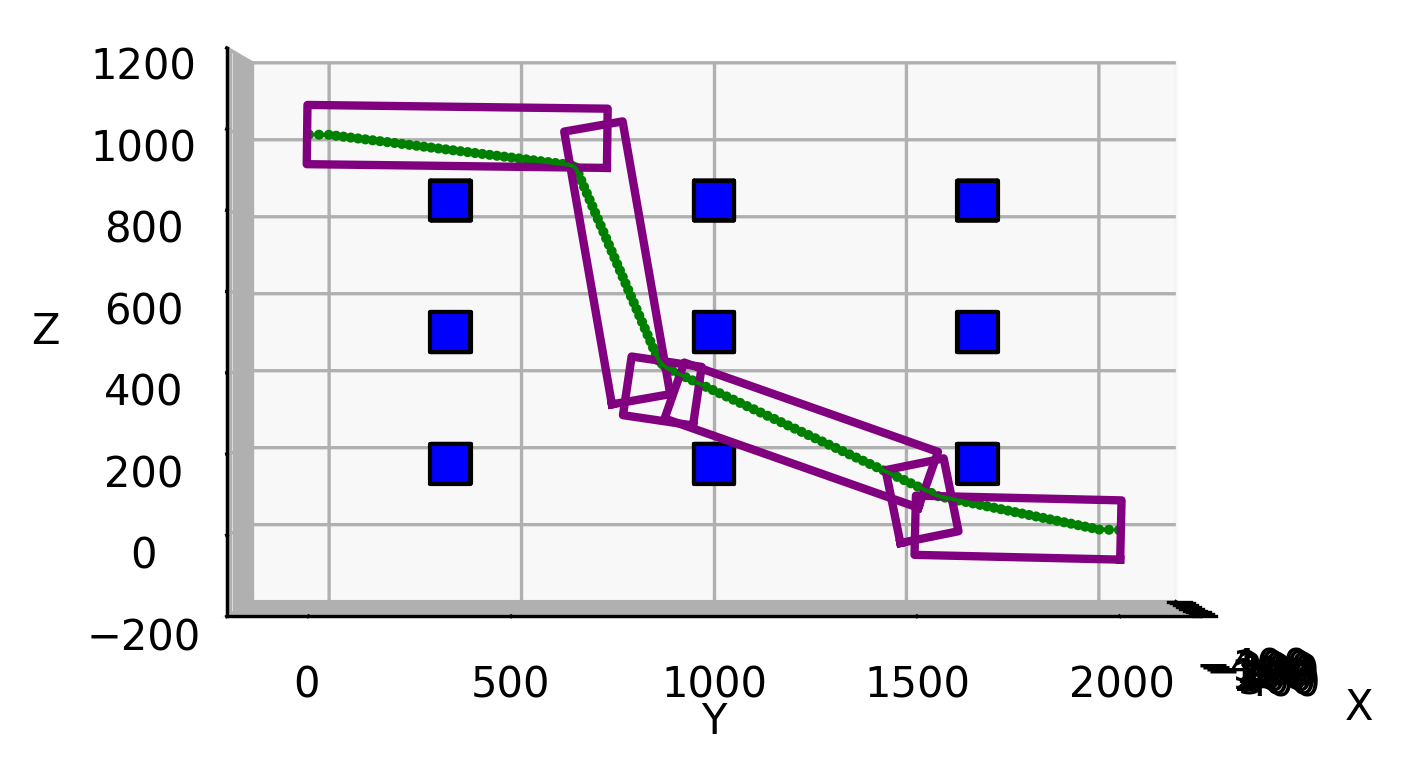
\includegraphics[width=0.95\linewidth]{figs/chap5/BadTrajectory/Bad Path.png}
    \caption{Safe flight corridor path though $3\times3$ grid, with a B-Spline path generated through it as a flight path reference trajectory. Due to the descending sections, the aircraft never follows the trajectory properly.}
    \label{fig:SFC_PathFollowing_failure}
\end{figure}

\section{Conclusion}

\subsection{Contributions}

This paper has discussed several contributions to general robotics research, with a particular emphasis on VTOL transition control.
The results from this thesis include the following key results:

\begin{itemize}
    \item The transition of a VTOL from hover to forward flight, and vice versa is a very complicated dynamic problem that has been researched extensively over that last several decades.
      Other solutions for VTOL transition usually use some switching criteria based on airspeed to slowly change from hover to fixed-wing flight.
      This paper develops the dynamics and controller for a 2D quadplane VTOL simplification.
      Specifically, it is shown that a 2D quadplane is a differentially flat sytem, so a differentially flat controller is implemented.
      This controller requires an input trajectory of position, velocity, and acceleration for all time samples.
      The pitch-free trajectory tracking controller finds the inertial frame force that will zero the state error.
      The pitch optimizer finds the optimal pitch to generate the most lift possible from the airframe; this causes the switch from hover to fixed-wing.
      The moment controller finds needed moment to control the aircraft to that specified pitch.
      Finally, the elevator and thrust allocators find the control inputs that produced the desired forces and moments.
      This controller is implemented on various reference trajectories, including landing. 
      With the exception of descending, this controller is able to accurately follow a system and transition from hover to fixed-wing flight without the need for gain scheduling.
    \item For a standard fixed-wing aircraft, there are thirty coefficients of aerodynamics, for lift, drag, and east forces, as well as $l$, $m$, and $n$ for roll pitch and yaw moments.
      A recursive LMS filter was developed for each set of coefficients and the corresponding flight data.
      Sensor data is gathered during a flight, including accelerometer data, gyroscope data, airspeed, and angle of attack.
      At each time sample, that data is processed through the each LMS filter and the coefficients are recursively estimated.
      The aircraft is subjected to specific maneuvers that excite phughoid and dutch roll modes, which produce large sensors signals to identify each coefficient.
      These manuevers and LMS filters were implemented in a fixed-wing simulation and proved the potential of aircraft coefficient estimation.
      Future implementations will be used to calibrate VTOL autopilots to have more accurate control.
    \item B-Splines form the basis of robotic trajectory planning. 
      The ability to efficiently generate and update B-Splines trajectories in real time is crucial for many robotic applications.
      B-Splines can be represented in 
\end{itemize}



\section{Future Work}

The autopilot framework is still in its infancy. There is much exciting work left to do for 

\subsection{Rosflight Integration}

Once a 3D controller is successfully developed in simulation for a quadplane, or another VTOL aircraft, the trajectory-following algorithm may be implemented in hardware. The BYU Magicc Lab is heavily investing time and resources into the development of open source autopilots developed on the ROS2 framework. These autopilot stacks are collectively known as Rosflight \ref{fig:RosflightLogo}. 

\begin{figure}
    \centering
    
\includegraphics[width=0.3\linewidth]{figs/chap5/rosflightLogo.png}
    \caption{ROSflight project illustration from the MAGICC Lab website. Image from Brigham Young University, 2026.}
    \label{fig:RosflightLogo}
\end{figure}

The best future for a hardware implementation of the differentially flat trajectory tracking controller is the development of a this as part of the larger Rosflight project. 

Rosflight also needs B-Splines.

\subsection{RViz and Unreal Simulation}

It goes without saying that our current simulation package is rather primitive. We have been using OpenGL in python for the simulation graphics for this aircraft. The graphics are rather grainy and unsophisticated. If this algorithm is integrated into Rosflight, updating these graphics would be greatly appreciated. 

\subsection{Real-Time RRT}

A primary assumption of the algorithm explained in Section \ref{ch:rrt_flight_corridors} is that the obstacle field is static, or that it does not change with time. This is useful for 


\cite{vtol_trajectory} 





